\section{Cobordism 2}
Suppose we have 
\begin{itemize}
\item a punctured Riemann sphere $M$

\item co-oriented link $\Lambda_0 = (\Phi_0,\xi_0)$ about $0$

\item co-oriented link $\Lambda_\infty = (\Phi_\infty,\xi_\infty)$ about $\infty$ 

\item a co-oriented lines $\Lambda_{squig} = (\Phi_{squig}, \xi_{squig})$ that refines the stratification induced by $\Lambda_0 \coprod \Lambda_\infty$ to a regular cell complex 
\end{itemize}
and suppose we have a nested disk $D' \subset D \subset M$ and a smooth chart
\[
	f: \{(x,z)\in \R^2 ~|~ x^2+z^2 < 4 \} \rightarrow D
\]
such that 
\begin{itemize}
\item $\{(x,z)\in \R^2 ~|~ x^2+z^2 < 1\}$ is mapped to $D'$ 

\item I will abuse the notation so that $D'$ denotes $\{(x,z)\in \R^2 ~|~ x^2+z^2 < 1\}$ and $D$ denotes $\{(x,z)\in \R^2 ~|~ x^2+z^2 < 4 \}$

\item $\{(x,z)\in D' ~|~ z = -\frac{5}{3}x^2 + \frac{3}{4} \}$, co-oriented downward, is mapped to $\Lambda_0 |_{D'}$

\item $\{(x,z)\in D' ~|~ z = \frac{1}{2} \}$, co-oriented upward, is mapped to $\Lambda_\infty |_{D'}$

\item $\{(x,z)\in D' ~|~ z=\sqrt{\frac{1}{16} - (z+\frac{1}{4})^2}, z > -\frac{5}{3}x^2 + \frac{3}{4} \} \coprod \{(x,z)\in D' ~|~ z=\sqrt{\frac{1}{16} - (z-\frac{1}{4})^2}, z > -\frac{5}{3}x^2 + \frac{3}{4} \}$, co-oriented downward, is mapped to $\Lambda_{squig} |_{D'}$
\end{itemize}
Suppose we have a sheaf $\mathfrak{F}$ singular supported on $\Lambda_0 \coprod \Lambda_\infty \coprod \Lambda_{squig}$, $f^*\mathfrak{F}$ is described as the following legible diagram.

\begin{definition}
\begin{align*}
s_0(sgn_1,sgn_2,sgn_3,sgn_4):=~ &\{(x,z) \in D' ~|~ sgn(z+\frac{5}{3}x^2 - \frac{3}{4})=sgn_1,~ sgn(\frac{1}{2}-z)=sgn_2,\\ 
&sgn((x+\frac{1}{4})+z^2 - \frac{1}{16})=sgn_3,~sgn((x-\frac{1}{4})+z^2 - \frac{1}{16})=sgn_4 \}
\end{align*}
where the $3^{rd}$ and the $4^{th}$ arguments are optional. Also, \begin{align*}
&s_0^+(sgn_1,sgn_2,sgn_3,sgn_4) := s_0(sgn_1,sgn_2,sgn_3,sgn_4) \cap \{(x,z)\in \R^2 ~|~ x>0\} \\
&s_0^-(sgn_1,sgn_2,sgn_3,sgn_4) := s_0(sgn_1,sgn_2,sgn_3,sgn_4) \cap \{(x,z)\in \R^2 ~|~ x<0\} \\
\end{align*}
\end{definition}

Note that $\Lambda_0 \coprod \Lambda_\infty \coprod \Lambda_{squig}$ divides $D'$ into $7$ regions which are
\[
	s_0(+,-,+,+),s_0(+,-,-,+),s_0(+,-,+,-),s_0(-,-),s_0^-(+,+),s_0^+(+,+),s_0(-,+)
\]

\textbf{Stalks:}
\begin{itemize}
\item $F_0(s_0(+,-,+,+))$ := $0$
\item $F_0(s_0(+,-,-,+))$ := $\C \xrightarrow{\times a} \C $
\item $F_0(s_0(+,-,+,-))$ := $\C \xrightarrow{\times b} \C $
\item $F_0(s_0(-,-))$ := $\C[-1]$
\item $F_0(s_0^-(+,+))$ := $\C$
\item $F_0(s_0^+(+,+))$ := $\C$
\item $F_0(s_0(-,+))$ := $0$
\end{itemize}

\textbf{Generization maps:}
\begin{itemize}
\item $F_0(s_0(0,-,+,+)):~ F_0(s_0(-,-))\rightarrow F_0(s_0(+,-,+,+))$ := zero map

\item $F_0(s_0(+,-,0,+)):~ F_0(s_0(+,-,-,+))\rightarrow F_0(s_0(+,-,+,+))$ := zero map

\item $F_0(s_0(+,-,+,0)):~ F_0(s_0(+,-,+,-))\rightarrow F_0(s_0(+,-,+,+))$ := zero map

\item $F_0(s_0^-(+,0,+,+)):~ F_0(s_0(+,-,+,+))\rightarrow F_0(s_0^-(+,+))$ := zero map

\item $F_0(s_0^+(+,0,+,+)):~ F_0(s_0(+,-,+,+))\rightarrow F_0(s_0^+(+,+))$ := zero map

\item $F_0(s_0^-(0,+)):~ F_0(s_0(-,+))\rightarrow F_0(s_0^-(+,+))$ := zero map

\item $F_0(s_0^+(0,+)):~ F_0(s_0(-,+))\rightarrow F_0(s_0^+(+,+))$ := zero map

\item $F_0(s_0(0,-,-,+)):~ F_0(s_0(-,-))\rightarrow F_0(s_0(+,-,-,+))$ := 
\begin{tikzcd}
\C \arrow[r, "id"]     & \C  \\
0 \arrow[r]\arrow[u,] & \C \arrow[u,"\times a"]
\end{tikzcd}

\item $F_0(s_0(0,-,+,-)):~ F_0(s_0(-,-))\rightarrow F_0(s_0(+,-,+,-))$ := 
\begin{tikzcd}
\C \arrow[r, "id"]     & \C  \\
0 \arrow[r]\arrow[u,] & \C \arrow[u,"\times b"]
\end{tikzcd}

\item $F_0(s_0(+,0,-,+)):~ F_0(s_0(+,-,-,+))\rightarrow F_0(s_0^-(+,+))$ := 
\begin{tikzcd}
\C \arrow[r,]     & 0  \\
\C \arrow[r, "id"]\arrow[u,"\times a"] & \C \arrow[u,]
\end{tikzcd}

\item $F_0(s_0(+,0,+,-)):~ F_0(s_0(+,-,+,-))\rightarrow F_0(s_0^+(+,+))$ := 
\begin{tikzcd}
\C \arrow[r,]     & 0  \\
\C \arrow[r, "id"]\arrow[u,"\times b"] & \C \arrow[u,]
\end{tikzcd}
\end{itemize}

Now I will define a cobordism of $f^*\mathfrak{F}$, say $Cobordism_2$ that satisfies the following conditions
\begin{itemize}
\item $Cobordism_2$ is supported on $overline{D}$

\item $Cobordism_2$ inside of $D-D'$ is perturbed so that $\Lambda$'s remain smooth link throughout the isotopy but won't exactly describe what it is

\item I will only describe $Cobordism_2$ inside $D'$
\end{itemize}
Now let's define $Cobordism_2$ as a legible diagram on $D'\times [0,1]_t$ whose regions are the regions separated by the following hyperplanes corresponding to the world sheets of $\Lambda_0$, $\Lambda_\infty$, and $\Lambda_{squig}$
\begin{itemize}
\item world sheet of $\Lambda_0$: 
$\{(x,z,t) \in D' \times [0,1] ~|~ z=-\frac{5}{3}(1-t)x^2 - \frac{5}{4}t+\frac{3}{4}\}$, where hairs are pointing downward. Note that when $t=t_0$, the above set is the parabola passing through $(-\frac{\sqrt{3}}{2}, -\frac{1}{2})$, $(\frac{\sqrt{3}}{2}, -\frac{1}{2})$, and $(0,-\frac{5}{4}t_0 + \frac{3}{4})$.

\item world sheet of $\Lambda_\infty$: 
$\{(x,z,t) \in D' \times [0,1] ~|~ z=\frac{1}{2} \}$, where hairs are pointing upward.

\item world sheet of $\Lambda_{squig}$:\\
$\{(x,z,t) \in D' \times [0,1] ~|~ z=\sqrt{\frac{1}{16}-(x+\frac{1}{4})^2,z>\frac{1}{2}, z>-\frac{5}{3}(1-t)x^2 - \frac{5}{4}t+\frac{3}{4}} \cup \{(x,z,t) \in D' \times [0,1] ~|~ z=\sqrt{\frac{1}{16}-(x-\frac{1}{4})^2},z>\frac{1}{2},z>-\frac{5}{3}(1-t)x^2 - \frac{5}{4}t+\frac{3}{4}\} \cup  \{ ~|~ x=0,z<\frac{1}{2},z>-\frac{5}{3}(1-t)x^2 - \frac{5}{4}t+\frac{3}{4}\}$, where hairs are pointing downward,downward,leftward for each component.
\end{itemize}
\begin{definition}
\begin{align*}
s(sgn_1,sgn_2,sgn_3,sgn_4)&:=~\{(x,z,t) \in D' \times [0,1] ~|~\\ &sgn(z+\frac{5}{3}(1-t)x^2 + \frac{5}{4}tx - \frac{3}{4})=sgn_1,~ sgn(\frac{1}{2}-z)=sgn_2,\\ 
&sgn((x+\frac{1}{4})+z^2 - \frac{1}{16})=sgn_3,~sgn((x-\frac{1}{4})+z^2 - \frac{1}{16})=sgn_4 \}
\end{align*}
where the $3^{rd}$ and the $4^{th}$ arguments are optional. Also, \begin{align*}
s^+(sgn_1,sgn_2,sgn_3,sgn_4) := &s(sgn_1,sgn_2,sgn_3,sgn_4) \cap \{(x,z)\in \R^2 ~|~ x>0\} \\
s^0(sgn_1,sgn_2,sgn_3,sgn_4) := &s(sgn_1,sgn_2,sgn_3,sgn_4) \cap \{(x,z)\in \R^2 ~|~ x<0\} \\
s^-(sgn_1,sgn_2,sgn_3,sgn_4) := &s(sgn_1,sgn_2,sgn_3,sgn_4) \cap \{(x,z)\in \R^2 ~|~ x<0\} \\
\end{align*}
\end{definition}
The above three world sheets separate $D'\times [0,1]$ into $7$ regions
\[
	s(+,-,+,+),s(+,-,-,+),s(+,-,+,-),s(-,-),s^-(+,+),s^+(+,+),s(-,+)
\]
and we get the following stratification
\begin{itemize}
\item $3$ dimensional strata: \\$s(+,-,+,+),s(+,-,-,+),s(+,-,+,-),s(-,-),s^-(+,+),s^+(+,+),s(-,+)$

\item $2$ dimensional strata: \\$s(0,-,+,+),s(+,-,0,+),s(+,-,+,0),s(0,-,-,+),s(0,-,+,-),s^-(+,0,+,+),$\\
$s^+(+,0,+,+),s(+,0,-,+),s(+,0,+,-),s(-,0),s^-(0,+),s^+(0,+),s^0(+,+)$

\item $1$ dimensional strata: \\$s(0,-,0,+),s(0,-,+,0),s(+,0,0,+),s(+,0,+,0),s^-(0,0),s^+(0,0),s^0(+,0),s^0(0,+)$

\item $0$ dimensional strata: \\ $s(0,0,0,0)$
\end{itemize}
Now let's define a legible diagram $F$ as follows\\
\textbf{Stalks:}
\begin{itemize}
\item $F(s(+,-,+,+))$ := $0$
\item $F(s(+,-,-,+))$ := $\C \xrightarrow{\times a} \C $
\item $F(s(+,-,+,-))$ := $\C \xrightarrow{\times b} \C $
\item $F(s(-,-))$ := $\C[-1]$
\item $F(s^-(+,+))$ := $\C$
\item $F(s^+(+,+))$ := $\C$
\item $F(s(-,+))$ := $0$
\end{itemize}

\textbf{Generization maps:}
\begin{itemize}
\item $F(s(0,-,+,+)):~ F(s(-,-))\rightarrow F(s(+,-,+,+))$ := zero map

\item $F(s(+,-,0,+)):~ F(s(+,-,-,+))\rightarrow F(s(+,-,+,+))$ := zero map

\item $F(s(+,-,+,0)):~ F(s(+,-,+,-))\rightarrow F(s(+,-,+,+))$ := zero map

\item $F(s^-(+,0,+,+)):~ F(s(+,-,+,+))\rightarrow F(s^-(+,+))$ := zero map

\item $F(s^+(+,0,+,+)):~ F(s(+,-,+,+))\rightarrow F(s^+(+,+))$ := zero map

\item $F(s^-(0,+)):~ F(s(-,+))\rightarrow F(s^-(+,+))$ := zero map

\item $F(s^+(0,+)):~ F(s(-,+))\rightarrow F(s^+(+,+))$ := zero map

\item $F(s(0,-,-,+)):~ F(s(-,-))\rightarrow F(s(+,-,-,+))$ := 
\begin{tikzcd}
\C \arrow[r, "id"]     & \C  \\
0 \arrow[r]\arrow[u,] & \C \arrow[u,"\times a"]
\end{tikzcd}

\item $F(s(0,-,+,-)):~ F(s(-,-))\rightarrow F(s(+,-,+,-))$ := 
\begin{tikzcd}
\C \arrow[r, "id"]     & \C  \\
0 \arrow[r]\arrow[u,] & \C \arrow[u,"\times b"]
\end{tikzcd}

\item $F(s(+,0,-,+)):~ F(s(+,-,-,+))\rightarrow F(s^-(+,+))$ := 
\begin{tikzcd}
\C \arrow[r,]     & 0  \\
\C \arrow[r, "id"]\arrow[u,"\times a"] & \C \arrow[u,]
\end{tikzcd}

\item $F(s(+,0,+,-)):~ F(s(+,-,+,-))\rightarrow F(s^+(+,+))$ := 
\begin{tikzcd}
\C \arrow[r,]     & 0  \\
\C \arrow[r, "id"]\arrow[u,"\times b"] & \C \arrow[u,]
\end{tikzcd}
\end{itemize}
\begin{proposition}
The above diagram is a well-defined legible diagram.
\end{proposition}
\begin{proof}
It is enough to show that the total complexes of the subdiagrams the above defined diagram associated to sub-penultimate dimensional strata.\\
\textbf{(\RN{1}) $1$ dimensional strata:}
\begin{itemize}
\item subdiagram associated to $s(0,-,0,+)$:\\
\begin{tikzcd}[row sep = 2cm, column sep=2.5cm]
     & s(+,-,+,+)  \\
s(+,-,-,+) \arrow[r, "{s(0,-,-,+)}"]\arrow[ur,"{s(+,-,0,+)}"] & s(-,-) \arrow[u,"{s(0,-,+,+)}"]
\end{tikzcd}
=
\begin{tikzcd}
&  & & 0  \arrow[dr] \\
& &  & & 0  \\
& \C \arrow[rr] \arrow[dr,"\times a"] \arrow[uurr] & & 0\arrow[uu] \arrow[dr] \\
& & \C \arrow[rr,"\times 1"'] \arrow[uurr] & & \C \arrow[uu]
\end{tikzcd}

\item subdiagram associated to $s(0,-,+,0)$:\\
\begin{tikzcd}[row sep = 2cm, column sep=2.5cm]
s(+,-,+,+)&  \\
s(-,-) \arrow[u, "{s(0,-,+,+)}"] & s(-,-) \arrow[l,"{s(0,-,+,-)}"]\arrow[ul,"{s(+,-,+,0)}"]
\end{tikzcd}
=
\begin{tikzcd}
& 0  \arrow[dl,"\beta"]& &  \\
0    & &  & \\
& 0 \arrow[dl]\arrow[uu]  & & \C \arrow[ll]\arrow[dl,"\times b"]\arrow[lluu]\\
\C \arrow[uu] & & \C\arrow[ll,"\times 1"']\arrow[lluu]  &
\end{tikzcd}

\item subdiagram associated to $s(+,0,0,+)$:\\
\begin{tikzcd}[row sep = 2cm, column sep=1.5cm]
     & s(+,-,+,+)\arrow[ld, "{s^-(+,0,+,+)}"]&  \\
s^-(+,+) & & s(+,-,-,+) \arrow[ll,"{s(+,0,-,+)}"]\arrow[lu,"{s(+,-,0,+)}"]
\end{tikzcd}
=
\begin{tikzcd}
 &0\arrow[rd]\arrow[ldd]& && \\
 && 0\arrow[ldd] && \\
\C  \arrow[dr] && \C  \arrow[ll,"\times 1"] \arrow[dr,"\times a"]\arrow[luu] && \\
& 0 &  & \C\arrow[ll]\arrow[luu]&
\end{tikzcd}

\item subdiagram associated to $s(+,0,+,0)$:\\
\begin{tikzcd}[row sep = 2cm, column sep=1.5cm]
     & s(+,-,+,+)\arrow[rd, "{s^+(+,0,+,+)}"]&  \\
s(+,-,+,-) \arrow[ru,"{s(+,-,+,0)}"]\arrow[rr,"{s(+,0,+,-)}"]& & s^+(+,+) 
\end{tikzcd}
=
\begin{tikzcd}
 &0\arrow[rd]\arrow[rdd]& && \\
 && 0\arrow[rdd] && \\
\C  \arrow[dr]\arrow[ruu]\arrow[rr] && \C   \arrow[dr,"\times a"] && \\
& \C \arrow[rr,"\times 1"]\arrow[ruu]&  & 0&
\end{tikzcd}
\end{itemize}
\end{proof}

\begin{figure}[H]
    \centering
    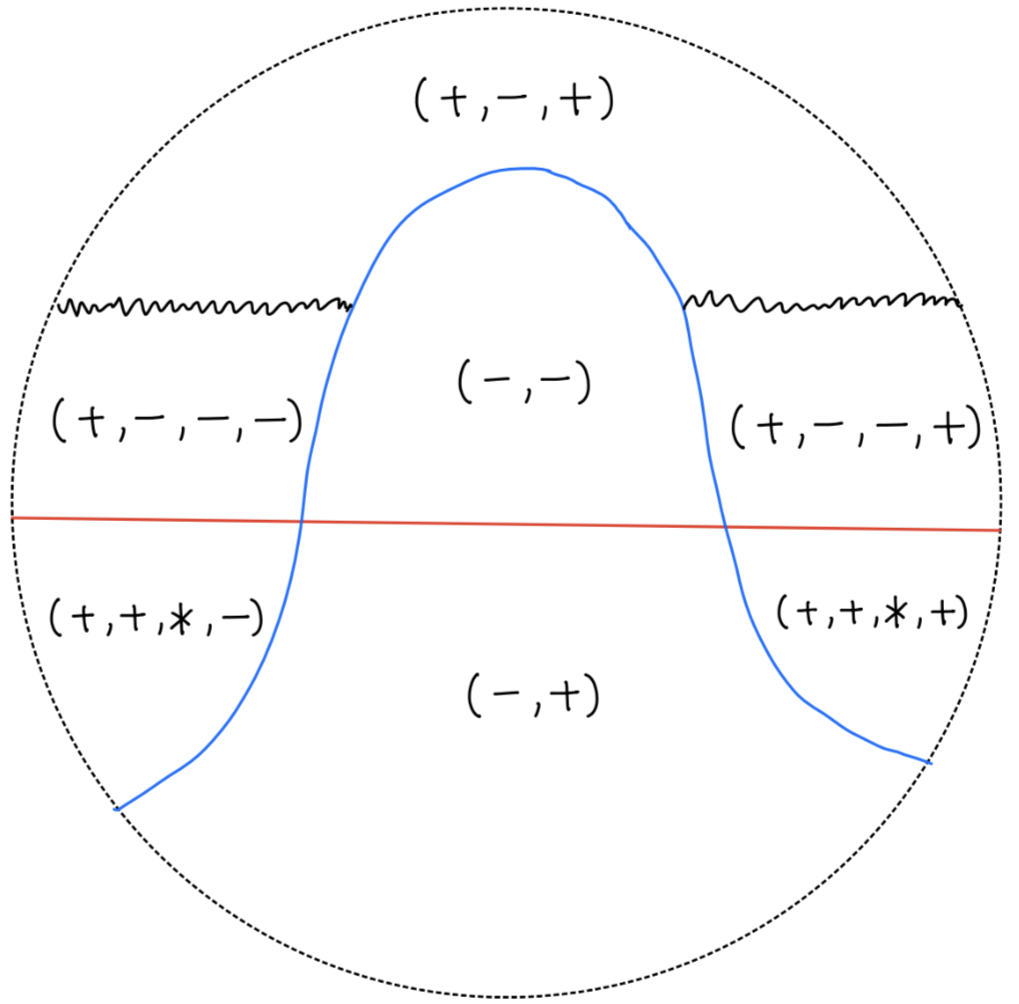
\includegraphics[scale = 0.95]{diagrams/lemma2/1.png} 
    \caption{Your caption here}
    \label{fig:your-label}
\end{figure}

\begin{figure}[H] 
    \centering
    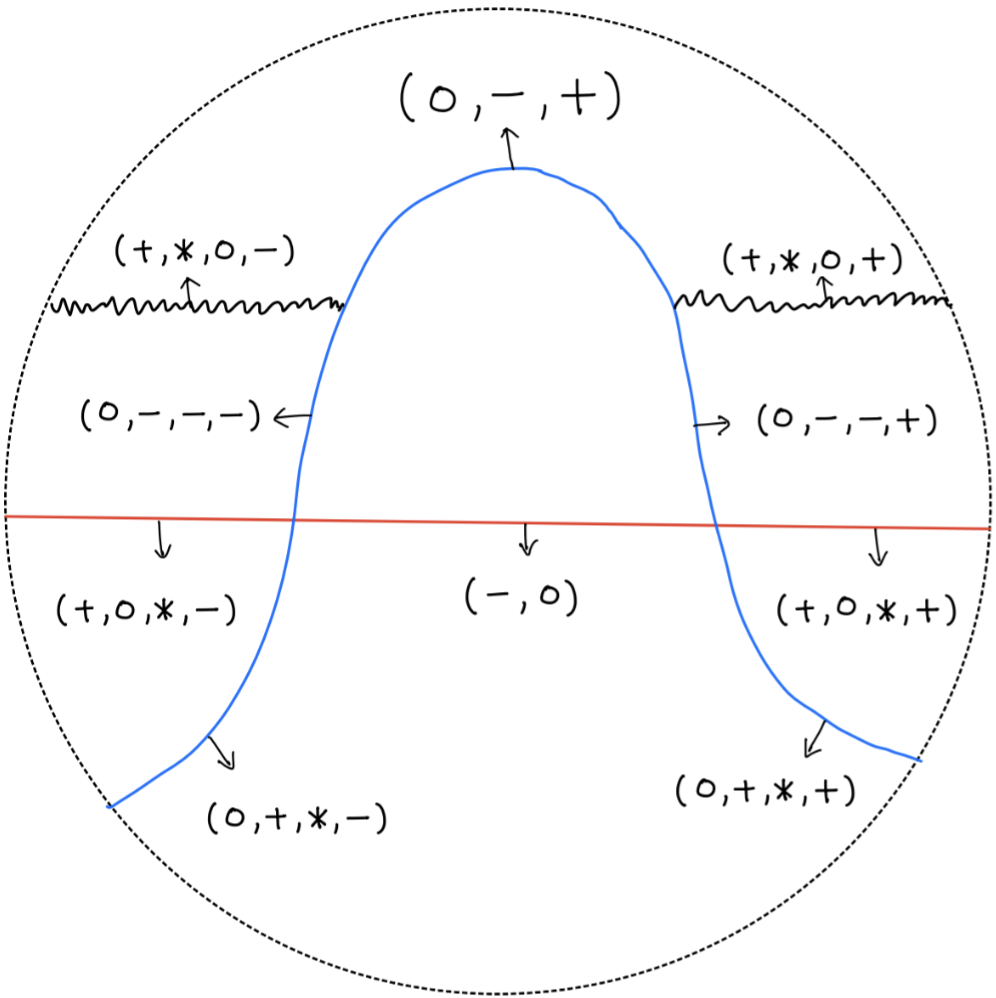
\includegraphics[scale = 0.95]{diagrams/lemma2/2.png} 
    \caption{Your caption here}
    \label{fig:your-label}
\end{figure}